\documentclass[preprint,12pt,authoryear]{elsarticle}

\usepackage{amsmath,amssymb}
\usepackage{booktabs}
\usepackage{graphicx}
\usepackage{multirow}
\usepackage{xcolor}
\usepackage{url}

\journal{Computers and Electronics in Agriculture}

\newcommand{\model}{Latent Neural ODE}
\newcommand{\todo}[1]{\textcolor{red}{[TODO: #1]}}

\begin{document}

\begin{frontmatter}

\title{Genotype- and temperature-conditioned plant growth prediction with latent neural ordinary differential equations under dense and sparse observations}

\author[inst1]{Author One}
\author[inst1]{Author Two}
\author[inst2]{Biology Collaborator}
\address[inst1]{\todo{Department, University, City, Country}}
\address[inst2]{\todo{Department, University, City, Country}}

\begin{abstract}
Predicting longitudinal plant growth across genotypes and environments requires a model that can represent nonlinear continuous dynamics without assuming that a single analytical growth equation is valid for every genotype. We present a genotype- and temperature-conditioned latent neural ordinary differential equation (Neural ODE) for plant growth trajectory prediction. A one-hot genotype representation and the temperature trajectory determine an initial latent state; a neural vector field then evolves this state continuously, and a decoder maps it to plant height or stem length. A weak genotype-specific logistic residual regularizes the learned trajectory without forcing the observed phenotype itself to follow logistic dynamics. We evaluate the approach on two contrasting datasets. The wheat experiment contains 19 genotypes measured in four field seasons and uses a protocol-matched year-held-out split. The external \textit{Arabidopsis thaliana} experiment contains nine genotypes, two temperature regimes, ten plants per genotype--temperature combination, and only four stem-length measurements per plant. After validation-only architecture and hyperparameter selection, a 1,655-parameter wheat model obtained a test root mean squared error (RMSE) of $0.03063\pm0.00062$~m over three seeds, compared with $0.05667\pm0.01274$~m for LSTM-NN and $0.06567\pm0.00306$~m for Logi-PINN. On the sparse Arabidopsis benchmark, the latent model obtained a test RMSE of $2.866\pm0.093$~cm, compared with random forest ($2.878\pm0.010$~cm), Logi-PINN ($2.987\pm0.126$~cm), and LSTM-NN ($2.951\pm0.064$~cm). Prediction figures are restricted to each sample's observed time span and do not display temporal extrapolation. These results support the use of latent continuous-time dynamics across species and suggest resilience to low temporal resolution. The Arabidopsis split evaluates new biological replicates within observed genotypes and temperature regimes; unseen-genotype and unseen-temperature validation remain future work.
\end{abstract}

\begin{keyword}
plant growth \sep plant height \sep latent neural ODE \sep physics-informed learning \sep genotype--environment interaction \sep sparse time series \sep Arabidopsis thaliana \sep wheat
\end{keyword}

\end{frontmatter}


\section{Introduction}
\label{sec:introduction}

Repeated phenotyping has shifted crop modelling from end-point prediction toward the analysis of complete growth trajectories. High-resolution imaging and sensor systems now quantify crop traits across space and time \citep{zhang2020phenotyping,kim2023monitoring,ehret2011tomato}, while time-series remote sensing and image-generation methods have enabled crop mapping and visual growth forecasting \citep{wang2021sentinel,drees2021brassica}. These measurements are valuable because plant growth is a dynamic response to genotype, development, and changing environmental conditions rather than a static trait. Nevertheless, longitudinal measurements remain expensive and irregular in many experiments, and measurements from different studies can range from daily field trajectories to only a few destructive or manual observations.

Machine learning has been applied widely to weather-conditioned crop prediction. Examples include wheat and maize yield forecasting from vegetation-index time series \citep{nagy2018forecasting}, farm-level and durum-wheat prediction \citep{tesfaye2021wheat,chergui2022durum}, hybrid performance prediction in corn \citep{sarijaloo2021corn}, and stacked recurrent models that combine unmanned-aerial-vehicle and meteorological time series \citep{wang2025sugarbeet}. Related studies have learned crop responses to temperature or limited climate information \citep{sharma2022evapotranspiration,singh2023eto}, grapevine phenology from climate records \citep{fasihi2025phenology}, and crop stress from biological signals \citep{wen2025stress}. Deep networks can also identify critical weather windows for spring wheat \citep{benke2025weather}, but purely data-driven models may require substantial data and can learn statistical shortcuts that are difficult to reconcile with biological growth.

Genotype--environment interaction further complicates temporal prediction. Multi-environment analyses must cope with incomplete genotype-by-environment matrices \citep{arciniegas2020imputation}, nonlinear interactions \citep{patil2023genotype}, and environmentally dependent genetic performance \citep{li2026plasticity}. The challenge is not limited to yield: greenhouse regulation, water use, morphology, and fresh biomass couple plant state to environmental forcing at multiple scales \citep{gao2024ipecm,salagovic2025tomato,zhang2026lettuce}. Consequently, a useful trajectory model should share information across genotypes while preserving genotype-specific responses and should incorporate environmental drivers without requiring an independent model for every genotype.

Hybrid mechanistic--machine-learning approaches offer one route to this goal. Process-model simulations have been assimilated with hyperspectral observations \citep{wang2025gecros}, combined with remote sensing and machine learning for wheat prediction \citep{kheir2025hybrid}, and synthesized with deep learning to estimate wheat biomass dynamics \citep{chen2026biomass}. Hybridization is especially appealing when training datasets are small \citep{dhal2022aquaponic}, when model parsimony matters \citep{saravi2021variable}, or when explanations are required \citep{ryo2022xai,ennaji2023nutrient}. Reservoir and pretrained sequence models provide additional options for vegetation-index forecasting \citep{olamofe2025ndvi}. Most directly, \citet{shao2026pinn} combined a logistic growth equation with an LSTM in a physics-informed neural network (Logi-PINN) for wheat plant-height prediction. Their results demonstrated the promise of weak biological constraints, but the observed height remained tied to a predetermined scalar logistic law whose adequacy can vary across genotype, environment, organ, and species.

Neural ordinary differential equations replace discrete hidden-state transitions with a learned continuous vector field \citep{chen2018neuralode}. Latent ODEs extend this idea by evolving an unobserved state that can represent richer dynamics than a single measured variable and are naturally compatible with irregular observation times \citep{rubanova2019latentode}. Augmenting the latent state can increase expressiveness and improve numerical behaviour \citep{dupont2019augmented}, while neural controlled differential equations formalize continuous-time responses to incoming covariates \citep{kidger2020neuralcde}. These ideas are complementary to physics-informed learning \citep{raissi2019pinn,karniadakis2021piml} and universal differential equations, which combine known and learned dynamics \citep{rackauckas2020ude}. Despite this methodological fit, latent continuous-time models have not been adequately tested for genotype-conditioned plant growth across both field-scale dense trajectories and extremely sparse external biological datasets.

This study develops a shared multiple-genotype \model{} that learns temperature-conditioned dynamics in a 16-dimensional latent state. A weak logistic residual is retained as a regularizer rather than imposed as the complete state equation. We make three contributions: (i) a continuous-time architecture that predicts an entire genotype-specific growth curve from genotype, calendar time, and a known temperature scenario, without using phenotype observations from the target trajectory; (ii) a year-held-out wheat evaluation aligned with the data processing of \citet{shao2026pinn}; and (iii) an external \textit{Arabidopsis thaliana} evaluation with only four observations per plant, designed to test whether the method remains useful in a low-time-resolution regime. The second dataset concerns primary inflorescence stem length rather than rosette area, thereby testing transfer across both species and growth traits.


\section{Materials and methods}
\label{sec:methods}

\subsection{Prediction task}

Let $g\in\{1,\ldots,G\}$ denote genotype, $T_g(t)$ an environmental temperature trajectory, and $y_g(t_i)$ plant height or stem length observed at a subset of times $\mathcal{O}_g$. The model predicts a complete trajectory $\hat y_g(t)$ on a common integration grid. Missing phenotype times do not contribute to the data loss. The principal task is trajectory-level generalization: to a held-out year for wheat and to new biological replicate plants for Arabidopsis. In both datasets, the evaluated genotype labels are present during training.

This implementation is an offline, scenario-conditioned predictor. The temperature trajectory over the prediction interval is assumed known and is read by the initial-state encoder. No height or stem-length observation from an evaluated trajectory is used as an input. It should therefore not be interpreted as a causal real-time forecast unless the encoder is restricted to past temperature observations.

\subsection{Genotype- and temperature-conditioned latent Neural ODE}

Each genotype is represented by a four-dimensional embedding $\mathbf e_g$ learned from a one-hot vector. An LSTM encoder reads standardized temperature and normalized calendar time in reverse temporal order and produces the initial latent state,
\begin{equation}
 \mathbf z_g(0)=E_{\phi}\!\left(\{T_g(\tau_j),\tau_j\}_{j=1}^{J},\mathbf e_g\right),
 \qquad \mathbf z_g(0)\in\mathbb R^{16}.
 \label{eq:encoder}
\end{equation}
The latent state evolves according to
\begin{equation}
 \frac{d\mathbf z_g}{d\tau}
 =3\tanh\!\left[f_{\theta}\!\left(\mathbf z_g(\tau),T_g(\tau),\mathbf e_g,\tau\right)\right],
 \qquad \tau\in[0,1],
 \label{eq:ode}
\end{equation}
where $f_{\theta}$ is a hyperbolic-tangent multilayer perceptron (MLP). The environmental value at intermediate solver stages is obtained by linear interpolation. A fixed-step fourth-order Runge--Kutta solver uses one substep per daily grid interval. Finally, an MLP decoder maps the latent trajectory to the phenotype,
\begin{equation}
 \hat y_g(\tau)=\operatorname{LeakyReLU}_{0.01}\!\left[D_{\psi}(\mathbf z_g(\tau))\right].
 \label{eq:decoder}
\end{equation}
For wheat, validation-only capacity tuning selected a 16-dimensional latent state, four-dimensional genotype embedding, one ODE hidden layer of width 16, decoder width 16, and LSTM encoder width 8, for 1,655 trainable parameters. For Arabidopsis, the external-validation experiment used the pre-tuning full-capacity instance: latent dimension 16, genotype embedding 4, two ODE hidden layers of width 32, decoder width 32, and encoder width 16, for 4,607 parameters. Thus, both experiments use the same continuous-time model and loss, while their capacity hyperparameters are reported separately.

\subsection{Weak logistic regularization}

The latent vector field is learned freely, but the decoded phenotype is weakly encouraged to resemble genotype-specific logistic growth. A parameter head maps the genotype embedding to
\begin{equation}
 r_g=\sigma(a_g), \qquad K_g=1+\tanh(b_g),
\end{equation}
where $r_g\in(0,1)$ and $K_g\in(0,2)$~m. The derivative of decoded height is calculated by the chain rule,
\begin{equation}
 \frac{d\hat y_g}{dt}
 =\frac{1}{d_{\tau}}\frac{\partial D_{\psi}}{\partial\mathbf z}
  \frac{d\mathbf z_g}{d\tau},
\end{equation}
where $d_{\tau}$ is the number of physical days represented by one normalized time unit. The physics residual is
\begin{equation}
 \mathcal L_{\mathrm{phys}}
 =\frac{1}{N J}\sum_{g,j}
 \left[
 \frac{d\hat y_g(t_j)}{dt}
 -r_g\hat y_g(t_j)\left(1-\frac{\hat y_g(t_j)}{K_g}\right)
 \right]^2.
 \label{eq:physics}
\end{equation}
Unlike a logistic ODE baseline, Eq.~\eqref{eq:physics} is a soft regularizer: the 16-dimensional neural vector field remains the trajectory-generating model.

The observed-data term is the mean of the per-trajectory masked RMSE,
\begin{equation}
 \mathcal L_{\mathrm{data}}
 =\frac{1}{N}\sum_{n=1}^{N}
 \sqrt{\frac{\sum_j m_{nj}(\hat y_{nj}-y_{nj})^2}
 {\sum_j m_{nj}}},
 \label{eq:data_loss}
\end{equation}
and the full objective is
\begin{equation}
 \mathcal L=\mathcal L_{\mathrm{data}}
 +2\mathcal L_{\mathrm{phys}}
 +0.1\,\frac{1}{N}\sum_n\left|\max_j\hat y_{nj}-K_{g(n)}\right|.
 \label{eq:loss}
\end{equation}
A monotonicity term and an explicit $r_g$ penalty were available but assigned zero weight in the reported configuration.

\subsection{Wheat field dataset and year-held-out protocol}
\label{subsec:wheatdata}

The wheat data originate from the Field Phenotyping Platform experiments described by \citet{roth2024thermal} and were processed following \citet{shao2026pinn}. Nineteen genotypes present in all four seasons (2018, 2019, 2021, and 2022) were retained. Height trajectories were aligned to a 285-day grid, and the first 115 positions were removed, leaving 170 daily positions. Missing positions before the first measurement were filled with the minimum observed height for that trajectory, as in the reference implementation. The only environmental channel in the reported experiment was 2-m air temperature, standardized using the training years.

The current model was trained on 88 plot-level trajectories from 2018 and 2019. Evaluation averaged replicate plots within each genotype--year combination, producing 38 training curves and 19 curves in each held-out year. Following split~0 of the reference GitHub implementation, model and hyperparameter selection used 2022, and the final test year was 2021. The current and reference models therefore use the same training, validation, and test years.

The model was optimized for 1,500 epochs with Adam, weight decay $10^{-4}$, and gradient clipping at 1.0. Validation RMSE was evaluated every ten epochs; checkpoint selection began after epoch 600 and used the mean of the ten most recent validation evaluations.

\subsubsection{Wheat capacity and hyperparameter selection}

All tuning decisions were made using validation RMSE from 2022; the 2021 test year was not used to rank configurations. First, ten capacity configurations varied latent dimension (4--16), genotype-embedding dimension (2--4), ODE width (8--32) and depth (one or two hidden layers), decoder width (8--32), and encoder width (4--16). Seeds 1 and 2 were used for screening. The Pareto candidates were then evaluated with learning rates $2\times10^{-3}$, $5\times10^{-3}$, and $10^{-2}$ and logistic-physics weights 0, 0.5, 2, and 5. The final architecture and hyperparameters were fixed before running seed 3. The reported three-seed wheat result therefore uses seeds 1--3, with latent dimension 16, genotype embedding 4, ODE width 16 and depth 1, decoder width 16, encoder width 8, learning rate $10^{-2}$, physics weight 2, and maximum-height weight 0.1. A 393-parameter micro model (latent dimension 4, genotype embedding 2, ODE width 8, decoder width 8, and encoder width 4) was retained as a reference-size efficiency ablation.

\subsection{Arabidopsis external low-time-resolution dataset}
\label{subsec:arabdata}

The external dataset was extracted from the supplementary workbook of \citet{naghani2024arabidopsis}. The response is primary inflorescence stem length, not whole-plant height or rosette area. It comprises nine genotypes (Col-0, \textit{phyB}, \textit{pif3}, \textit{pif4}, \textit{pif7-1}, \textit{pif7-2}, \textit{pif3 pif7}, \textit{pifq}, and 35S::PIF4), two temperature regimes, and ten plants per genotype--temperature combination. Plants were grown under long days (16-h light/8-h dark). The normal ambient-temperature regime (nAT) was 21/18~$^{\circ}$C day/night, and the high ambient-temperature regime (hAT) was 28/24~$^{\circ}$C day/night. Mean day/night temperature was used as the environmental input.

Each of the 180 plants has only four measurements: 29, 36, 39, and 49 days after sowing (DAS) under nAT and 27, 30, 37, and 41 DAS under hAT, for 720 measurements in total. All trajectories were represented on a common 27--49 DAS integration grid, but only the four observed dates contributed to the loss and metrics. Plant identifiers 1--6 were used for training, 7--8 for validation, and 9--10 for testing. Neural models were trained on 108 individual-plant curves. Validation and test metrics were computed on 18 replicate-averaged genotype--temperature curves, each with four observed points. Thus, the split measures generalization to new biological replicates under observed genotypes and temperature regimes; it does not test unseen genotypes or temperatures.

The Arabidopsis \model{} used the full-capacity architecture specified above and the same objective as wheat, with $d_{\tau}=22$ days. It was trained for 1,500 epochs from seeds 1--3. Checkpoint selection started at epoch 300 and used a ten-evaluation moving average of validation RMSE. The extremely sparse phenotype mask makes this dataset an external low-time-resolution test, although it does not by itself establish general robustness to every missingness pattern.

\subsection{Baselines and evaluation}

For wheat, we use the multiple-genotype one-hot LSTM-NN and Logi-PINN results reported by \citet{shao2026pinn} and preserved in the accompanying GitHub outputs. For Arabidopsis, the following models were fitted under the same plant split: genotype-specific logistic ODE, the paper's temperature-response ODE, random forest, the reference one-hot LSTM-NN, and Logi-PINN. Logistic $r_g$ and $K_g$ values were first fitted using training plants only and used to initialize Logi-PINN. To stabilize optimization, the prediction network used learning rate $10^{-3}$, the direct genotype-specific ODE parameters used $10^{-4}$, and the ODE parameters were frozen during a 500-epoch data-only warm-up.

The primary metric is trajectory-level RMSE: RMSE is calculated separately over the observed points of each replicate-averaged trajectory and then averaged across trajectories, matching the convention of \citet{shao2026pinn}. Mean absolute error (MAE) is reported for Arabidopsis as a complementary measure. Neural models and random forest were evaluated with seeds 1--3, and values are reported as mean $\pm$ sample standard deviation across these three seeds. Logistic and temperature-informed ODE baselines are deterministic least-squares fits and were run once; manufacturing a seed variance for these models would not be meaningful. All prediction plots are clipped to the interval from the first actual observation to the last actual observation of the displayed sample. Curves between observations are interpolated model trajectories; no curve is shown outside the observed time span.


\section{Results}
\label{sec:results}

\subsection{Wheat: year-held-out plant-height prediction}
\label{subsec:wheatresults}

The tuned 1,655-parameter \model{} obtained train, validation, and test RMSEs of $0.02244\pm0.00019$, $0.03804\pm0.00067$, and $0.03063\pm0.00062$~m, respectively (Table~\ref{tab:wheat}). Relative to the original 4,647-parameter model, tuning reduced parameter count by 64.4\% while lowering mean validation and test errors. The 393-parameter micro model remained competitive at $0.03290\pm0.00141$~m test RMSE and was smaller than both reference networks. The tuned model reduced mean test RMSE by 46.0\% relative to LSTM-NN and 53.4\% relative to Logi-PINN under the matched year split.

\begin{table}[t]
\centering
\caption{Wheat multiple-genotype results under the matched year split: training on 2018/2019, validation on 2022, and testing on 2021. Values are mean $\pm$ sample standard deviation over seeds 1--3. RMSE is in metres. Reference rows were recalculated from the first three seed rows in the accompanying GitHub outputs.}
\label{tab:wheat}
\begin{tabular}{lrrrr}
\toprule
Model & Parameters & Train RMSE & Validation RMSE & Test RMSE \\
\midrule
\textbf{Tuned \model{} (ours)} & \textbf{1,655} & $\mathbf{0.02244\pm0.00019}$ & $\mathbf{0.03804\pm0.00067}$ & $\mathbf{0.03063\pm0.00062}$ \\
Micro \model{} & 393 & $0.02473\pm0.00064$ & $0.04153\pm0.00387$ & $0.03290\pm0.00141$ \\
Original \model{} & 4,647 & $0.02309\pm0.00063$ & $0.04210\pm0.00252$ & $0.03163\pm0.00021$ \\
LSTM-NN (reference) & 451 & $0.03433\pm0.00058$ & $0.07400\pm0.01044$ & $0.05667\pm0.01274$ \\
Logi-PINN (reference) & 463 & $0.03433\pm0.00252$ & $0.06633\pm0.00321$ & $0.06567\pm0.00306$ \\
\bottomrule
\end{tabular}
\end{table}

\begin{figure*}[t]
\centering
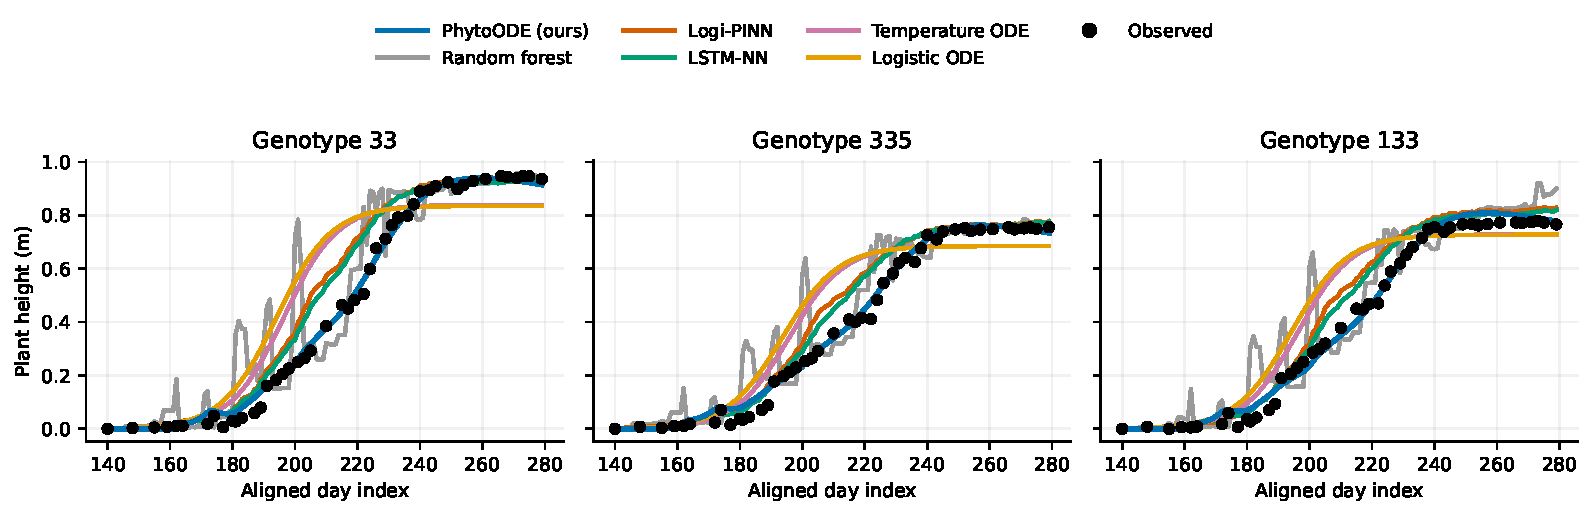
\includegraphics[width=0.96\textwidth]{figures/wheat_test_curves_no_extrapolation.pdf}
\caption{Wheat predictions in the held-out 2021 season for three genotypes selected with a fixed random seed. Black points are replicate-averaged actual observations. Blue lines and bands show the mean $\pm$ one standard deviation over seeds 1--3 of the tuned \model{}. For each genotype, the prediction is plotted only from its first actual observation to its last actual observation; temporal extrapolation is not shown.}
\label{fig:wheatcurves}
\end{figure*}

Figure~\ref{fig:wheatcurves} shows that the compact model captured genotype-dependent onset, rapid elongation, and plateau height within the measured interval. The displayed curves deliberately end with the data. Consequently, the figure evaluates trajectory reconstruction and year-held-out prediction over observed time support, not forecasting beyond the final phenotyping date.

\subsection{Arabidopsis: external validation with four observations per plant}
\label{subsec:arabresults}

The \model{} achieved the lowest mean test RMSE on the Arabidopsis primary-stem dataset, $2.866\pm0.093$~cm (Table~\ref{tab:arabidopsis}). This was marginally (0.4\%) lower than random forest and 4.1\% and 2.9\% lower than stabilized Logi-PINN and LSTM-NN, respectively. The result is notable because each plant contributed only four observed time points. In contrast, the two fixed-form process baselines had substantially larger errors, with test RMSEs of 4.121~cm for the temperature-informed ODE and 5.179~cm for the logistic ODE.

\begin{table}[t]
\centering
\caption{Arabidopsis primary inflorescence stem-length results under the plant-held-out split. Errors are in centimetres. Neural and random-forest values are mean $\pm$ sample standard deviation over seeds 1--3. Deterministic ODE fits were run once and therefore have no seed standard deviation.}
\label{tab:arabidopsis}
\begin{tabular}{lrrrr}
\toprule
Model & Train RMSE & Validation RMSE & Test RMSE & Test MAE \\
\midrule
\model{} (ours) & $1.401\pm0.088$ & $3.246\pm0.006$ & $\mathbf{2.866\pm0.093}$ & $2.463\pm0.088$ \\
Random forest & $0.153\pm0.018$ & $\mathbf{3.217\pm0.008}$ & $2.878\pm0.010$ & $\mathbf{2.347\pm0.001}$ \\
Logi-PINN & $1.721\pm0.034$ & $3.316\pm0.075$ & $2.987\pm0.126$ & $2.523\pm0.063$ \\
LSTM-NN & $1.701\pm0.122$ & $3.343\pm0.103$ & $2.951\pm0.064$ & $2.501\pm0.026$ \\
Temperature-informed ODE (single fit) & $3.678$ & $4.174$ & $4.121$ & $3.500$ \\
Logistic ODE (single fit) & $4.944$ & $5.274$ & $5.179$ & $4.502$ \\
\bottomrule
\end{tabular}
\end{table}

Random forest obtained the lowest MAE, outperforming the \model{} by 0.116~cm, while its mean RMSE was 0.012~cm higher. Thus, the RMSE difference between these models is small relative to biological variability and should not be interpreted as categorical superiority. The very low random-forest training error also indicates substantially greater interpolation capacity than its test performance would imply.

Condition-stratified analysis gave \model{} RMSEs of $2.144\pm0.050$~cm under nAT and $3.588\pm0.199$~cm under hAT. Random forest was better under hAT ($3.342\pm0.032$~cm) but worse under nAT ($2.414\pm0.037$~cm). The hAT trajectories begin and terminate earlier and often approach a plateau by 41 DAS, making their timing difficult to infer from four observations. Figure~\ref{fig:arabcurves} illustrates Col-0 predictions under both temperature regimes. All curves between observed points are model-based interpolation, not additional biological observations.

\begin{figure*}[t]
\centering

\includegraphics[width=0.96\textwidth]{figures/arabidopsis_col0_no_extrapolation.pdf}
\caption{Col-0 test observations and predictions under normal (nAT) and high (hAT) ambient temperature. Black points are means of the two held-out test plants. Stochastic-model lines are averages over seeds 1--3; ODE baselines are deterministic fits. Each line is clipped to the condition-specific interval between the first and last observation (nAT: 29--49 DAS; hAT: 27--41 DAS), so no temporal extrapolation is displayed.}
\label{fig:arabcurves}
\end{figure*}

Taken together, the Arabidopsis results support resilience to low temporal resolution in a species and organ distinct from the wheat development dataset. However, this evidence is bounded: all nine genotypes and both temperature regimes occur in training, validation, and test splits, and each test curve averages only two plants. The experiment therefore supports cross-species, sparse-trajectory applicability but not genotype or environmental extrapolation.


\section{Conclusion}
\label{sec:conclusion}

We introduced a genotype- and temperature-conditioned latent Neural ODE for predicting plant growth trajectories. The model learns continuous dynamics in a latent space while retaining a weak logistic growth residual. In wheat, validation-only tuning reduced model size from 4,647 to 1,655 parameters and produced a three-seed year-held-out test RMSE of $0.03063\pm0.00062$~m. A 393-parameter micro model remained substantially more accurate than the similarly sized reference LSTM-NN and Logi-PINN. In an external Arabidopsis primary-stem dataset with only four measurements per plant, the latent model achieved a three-seed test RMSE of $2.866\pm0.093$~cm, marginally lower than random forest and lower than LSTM-NN and Logi-PINN. The combination of dense field data and sparse controlled-environment data suggests that latent continuous-time dynamics can provide a useful common representation across species, organs, and temporal resolutions.

Three limitations define the next experiments. First, capacity and hyperparameters were tuned on one wheat validation year; the fixed selected configuration should be evaluated over the other five year combinations without test-year retuning. Second, the Arabidopsis split holds out plants rather than genotypes or temperature regimes. Independent growth cohorts with more biological replicates, genotype-held-out validation, intermediate or fluctuating temperature treatments, and targeted sampling around bolting and rapid elongation would provide a stronger test of biological generalization. Third, the present evaluation and figures are restricted to measured temporal support and do not establish accuracy beyond the last phenotyping date. A causal forecasting variant should restrict the environmental encoder to temperatures available up to the forecast origin and evaluate explicitly defined extrapolation horizons.

\section*{Data and code availability}
\todo{Add public repository URL, software environment, model checkpoints, processed-data scripts, and permanent identifiers for both datasets.}

\section*{Declaration of competing interest}
The authors declare that they have no known competing financial interests or personal relationships that could have appeared to influence the work reported in this paper.

\section*{Acknowledgements}
\todo{Add funding, facility, and collaborator acknowledgements.}

\bibliographystyle{elsarticle-harv}
\bibliography{references}

\end{document}
